\documentclass{article}

\usepackage{amsmath}
\usepackage{tikz}
\usepackage{graphicx}

\title{Turing Machine Documentation}
\author{Ryan Peruski, Maria Hernandez}
\date{\today}

\begin{document}

\maketitle
\section{Roles}

\begin{itemize}
    \item \textbf{Ryan Peruski}: Created initial stack design and initial templates for the documentation. Revised the machine's design and suggested improvements. Added examples and revisions to the documentation.
    \item \textbf{Maria Hernandez}: Edited the stack design to adapt to the specific problem of "valid parentheses". Added string parsing, character constant parsing, and multi-line comments sections
    to both the TM and the documentation. Added examples and filled out much of the documentation.
\end{itemize}

\section{Definition}
This Turing Machine inputs any C-code and places opening parentheses, square brackets, curly brackets, or opening multi-line comment symbols on the stack and pop their respective closing operators. If the machine encounters a closing operator and 
it does not see the matching operator of the right type on the top of the stack (represented by the first blank to the right), 
it rejects. If the Turing Machine finishes reading the input and there is something on the stack, it will reject. 
If the original input is empty, it will accept. The machine will accept if it reads all input successfully and the stack is empty at the end.

In addition, this Turing Machine pseudo-parses strings and constant characters, by applying certain syntax rules explained below. 

\section{States, Transitions, Image}
The Turing machine operates by moving between states and performing transitions on the tape. The states and transitions are labeled as follows:

\begin{itemize}
    \item $Red:$ Reject states ($q_{reject}$)
    \item $Green:$ Accept state ($q_{accept}$)
    \item $Blue:$ Single quotes parsing
    \item $Pink:$ Double quotes parsing
    \item $Cyan:$ Stack's push states  
    \item $LightCoral:$ Stack's pop states
    \item $Purple:$ Multi-line comments section 
    \item $Black:$ Initial states to set up the $\#$
    \item $Beige:$ Transition state (between stack push operations, pop operations, single quotes and double quotes parsing, and multi-line comments)
    \item $Gray:$ State to determine the validity of the original input tape
\end{itemize}

Finally, the Turing Machine is shown in Figure\ \ref{fig: Turing Machine Pseudo-Parser}.
\begin{figure}[h]
    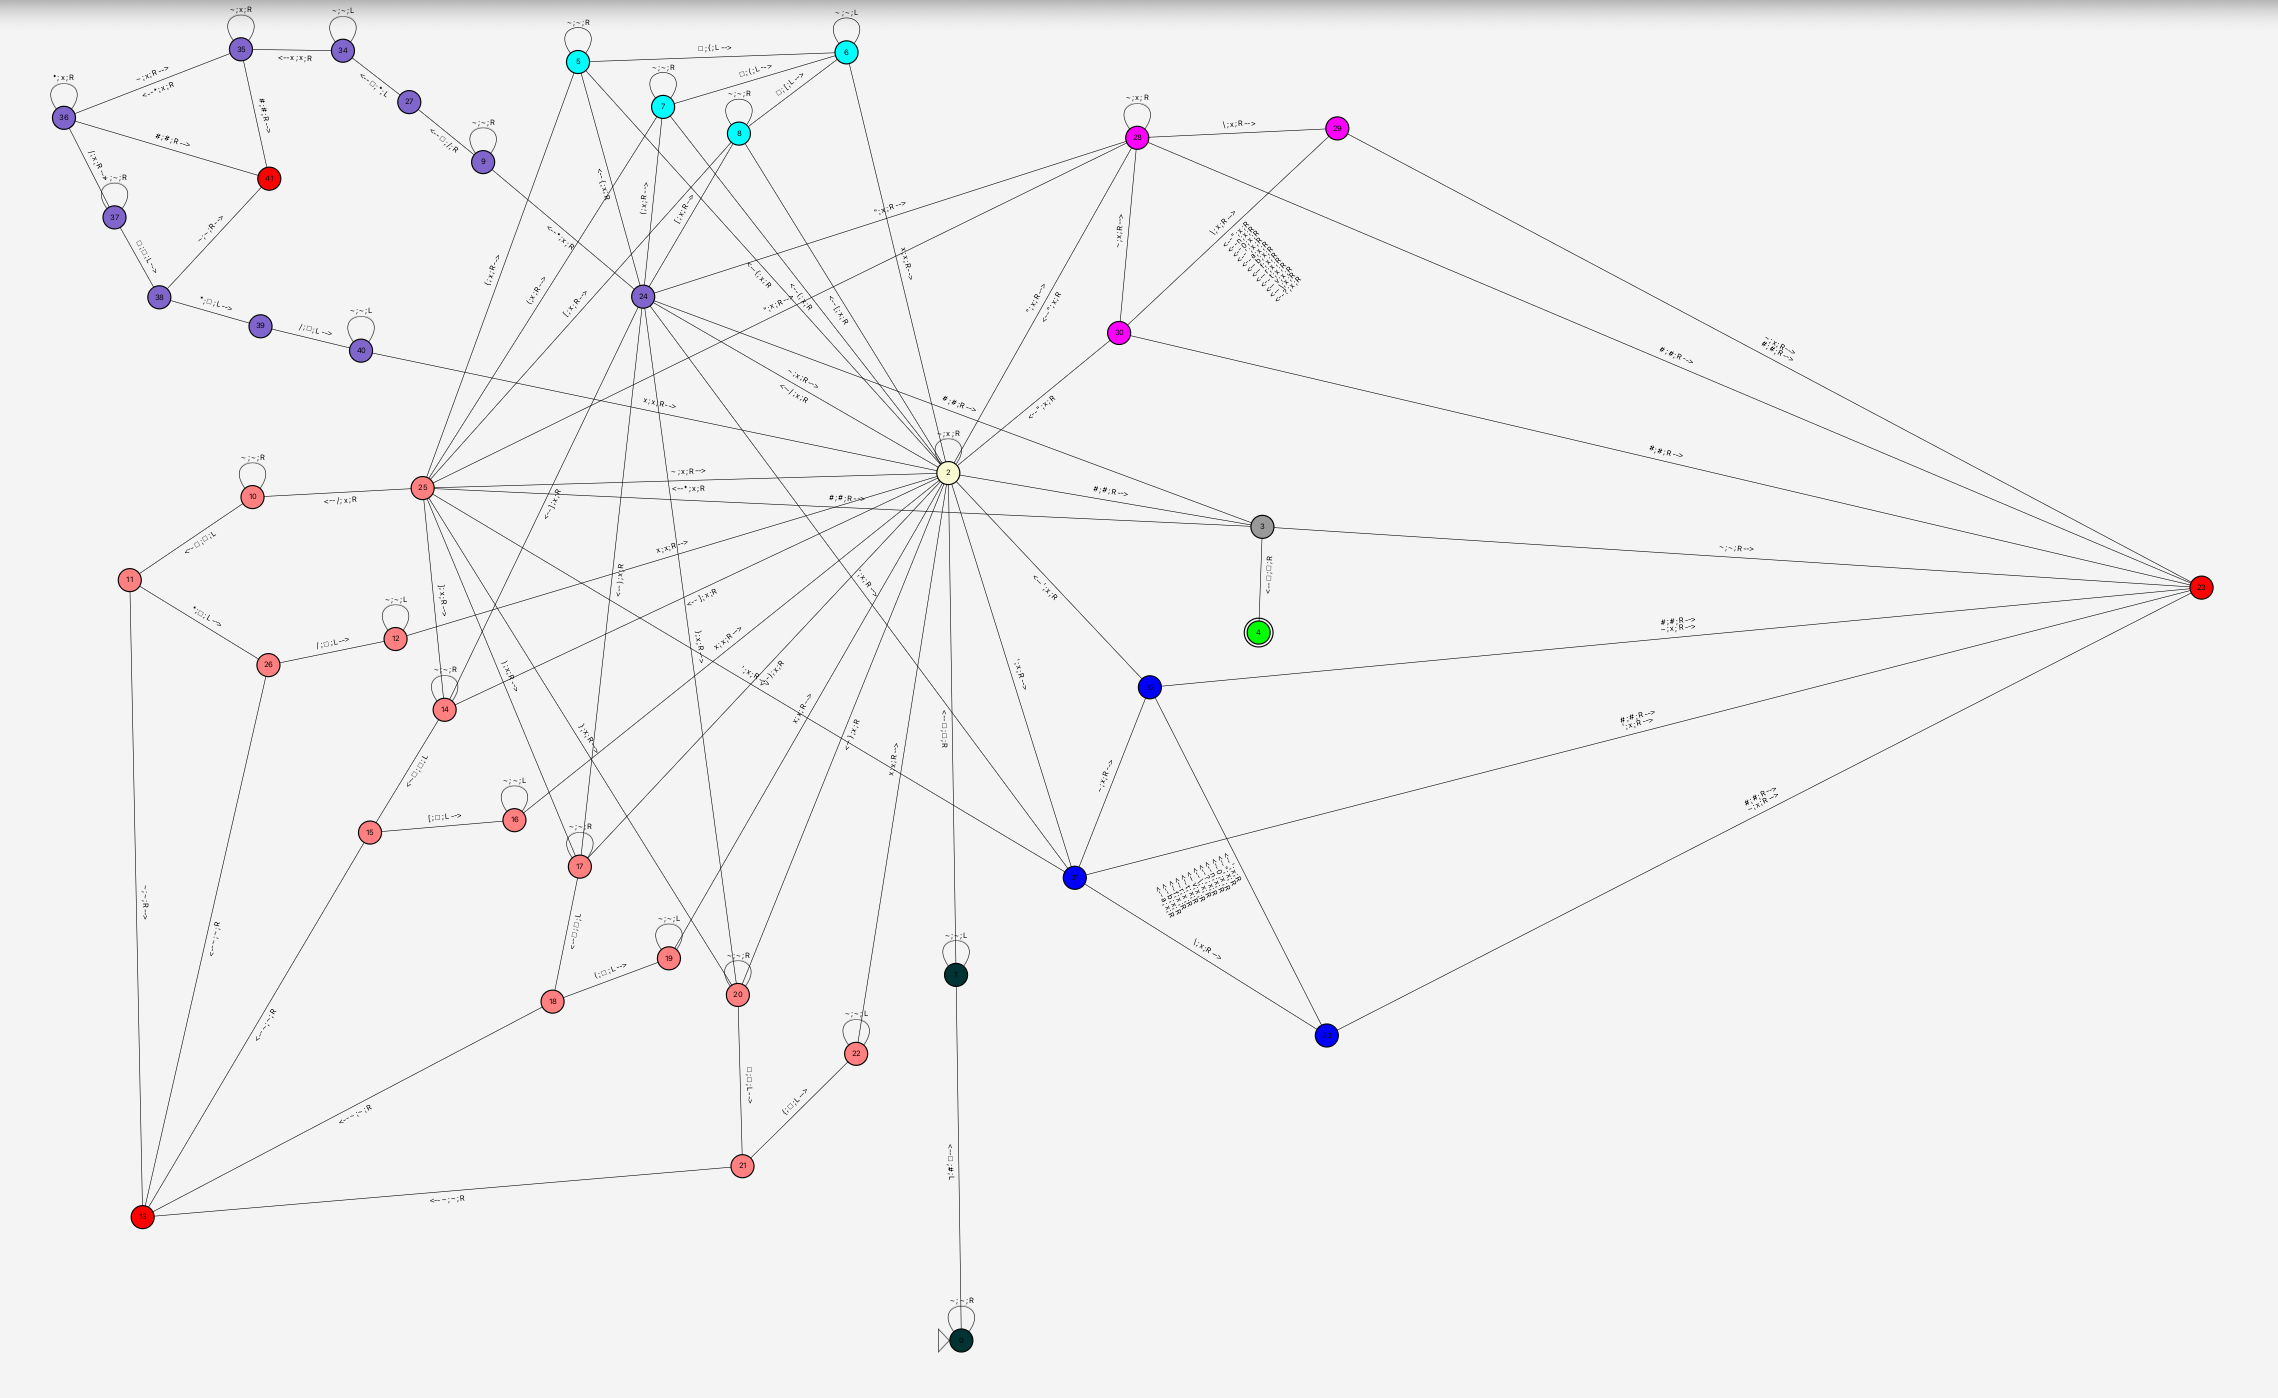
\includegraphics[width=\linewidth]{TuringMachineParser.png}
    \caption{Turing Machine.}\label{fig: Turing Machine Pseudo-Parser}
\end{figure}


\section{Machine Specifications}

\begin{itemize}
    \item Input alphabet: Any ASCII symbol, except $\#$, x, and space
    \item Tape alphabet:  Any ASCII symbol, including $\#$, x, and space
\end{itemize}

\subsection{Characters reserved for the tape alphabet}
The following are reserved characters: $\#$, x, and spaces. They are part of the tape alphabet, but they cannot be part of the 
input alphabet. $\#$ is reserved to delimit the end of the original input data. As soon as the machine starts running, it will mark the 
end of the original input data. x is reserved to mark the characters that have already been read from the original input data. 
Spaces are reserved to know the following: 1. Where to place the $\#$, 2. Where to start reading the original input data (after placing 
the $\#$ and going back), 3. Whether the stack is empty or not after finishing reading the original input data.

The tape will be divided by a $\#$. Anything before the $\#$ represents the original input data (code), and everything after the 
# represents the stack. 

In other words, the tape will use the structure: 
(original input data)$\#$(stack)

\subsection{How to start the machine}
In the original tape, the user may enter any character belonging to the input alphabet (aside from a space, #, or x). 
The start state is the state 0. The first operation the machine will do is to place the $\#$ to delimit the end of the 
original input data (usually C-code) and the beginning of the "stack". The only elements that can be placed on the stack are the opening 
operators -- namely, (,$\{$,[,/* 

\section{Functional Description of the Turing Machine}

\subsection{Valid (,),[,],$\{$,$\}$}
As previously mentioned, the TM evaluates whether the (,$\{$,[ characters in the original input data have their corresponding closing ],$\}$,) using stack operations (push for the left ones, pop for the right ones). 
There is an exception when these characters are either inside double quotes or inside  multi-line comments /**/. For instance, the machine will 
accept /*$\{$*/ and ")". This is because, in C, anything inside /**/ is ignored, and anything can be written inside "".

\subsection{Double quote section ""}
This TM is not only evaluating the parity of "", but also other syntax properties of C. If the original input data contains double quotes, 
the only way the machine will accept it is if it has an even number of double quotes. Namely, it accepts if after opening a double quote and writing 
any character in the string, the TM finds the respective closing double quote -– the only way to ensure this is if the machine goes back to state 2. 
There is an exception to this rule: the TM may accept an uneven number of " only if some of them are preceded by a \verb|\| (escape character). 
After the escape character, only certain characters are allowed (",n,0,', a,b,f,r,t,v,\,?). Note that we did not account for escape sequences for octal 
numbers \verb|\000| and hexadecimal numbers \verb|\xhh| since that would have made the TM needlessly complicated.

If the TM is currently at state 28 and it reads a $\#$, the original input data must have an uneven number of ", hence the machine rejects the string (ex: "Hello""). 
If the TM reads an escape character in state 28, it goes to state 29. If the TM is at state 29 and the following character in the tape is not any of 
the special sequence characters or if there are no more characters from the initial data (next character is $\#$), then the machine rejects the string 
(ex: "\verb|\k|, "\verb|\|). State 30 allows the TM to either read a new escape character \verb|\|, go back to state 2 -- if reading a closing ", read any other character
on the string, or reject the string if reading a $\#$. 

\subsection{Single quote section}

This TM is not only evaluating the parity of ', but also other syntax properties of C, including not accepting an empty character '' or only accepting certain escape 
sequence characters (the same ones that double quotes accept). The only way to accept an input containing single quotes is if it contains an opening and closing '. 
An uneven number of ' may be accepted if ' is preceded by an escape character. Even though the usage of multi-character constants is not strictly prohibited in C,
functions like "putc" are designed to output only a single character. Hence, when including multi-characters in '', "putc", for instance, will likely just output the 
lowest byte of the integer (assuming the machine is little endian). Due to this behavior, we are restricting our machine to only accept one character (maximum two if the 
input data includes the escape sequence) between ''. If while in state 31, the machine reads a $\#$ (end of original input data), or a ', the machine rejects it because 
either there is an opening ' without its corresponding closing ', or because it is an empty character. If while in state 32, the machine reads another character 
other than the closing ', the machine rejects the input. This machine does not allow multiple characters inside ''. 

\subsection{Comments}

The operators that gave us the most work were /* and */. Since the machine reads one character at a time, we needed to take into account several possible scenarios 
so that the machine always halts and correctly behaves in cases when the original tape has something like *{/}, or /(*), or, *(*), or *[/$\}$ (reject in this case). 
Also, we needed a special branch (purple branch) for the comments so that we could 
ignore everything inside /* */.

If the TM reads a / followed by a *, it writes an x and then places the / and * on the “stack” section. Then, the machine goes back and writes an x over all characters 
until reading both a * followed by a /. The machine rejects if, while reading characters, it finds the end of the original input data $\#$ before finding */ 
(ex: $\#$: /*Hello$\#$, /*Hello*$\#$, /*Hello***$\#$). If the TM reads a */ in the original input data and does not find the corresponding opening 
/* in the stack section, it rejects (ex: */$\#$, Hello*/$\#$). If the TM finds nested comments, it rejects (ex: /*/**/*/$\#$, /*/*****H**i*/*/). In this case, the /* inside /**/ 
is considered a comment, and thus, it is ignored. Consequently, the last */ will not have its corresponding opening /*. Everything inside the comments is ignored, hence, in this 
case, the TM allows single $\{$,[,(,),],$\}$. 

To be able to correctly implement the comments, this machine needs to find two consecutive characters in the input tape. Thus, this TM accounts for cases when it reads from the input tape a single * or a single / immediately followed by one of the other special characters  $\{$,[,(,),],$\}$,”,’,$\#$.
This is why states 24 and 25 have several transitions -- to account for cases like *(*), or *[/$\}$.

\section{Examples}
Here are some examples of input and output for the Turing machine:
\begin{itemize}
    \item \begin{verbatim} Input: v[i]=a[i][j];, Output:  xxxxxxxxxxxxx#, ACCEPTS \end{verbatim}
    \item \begin{verbatim} Input: for(;;)break;, Output:   xxxxxxxxxxxxx#, ACCEPTS \end{verbatim}
    \item \begin{verbatim} Input: {x=7}, Output:  xxxxx#, ACCEPTS \end{verbatim}
    \item \begin{verbatim} Input: for(i=0;i<v.size();i++)v[i]=2;, 
    Output: xxxxxxxxxxxxxxxxxxxxxxxxxxxxxx#, ACCEPTS \end{verbatim}
    \item \begin{verbatim} Input: v[i]=a[i, Output:  xxxxxxxx#[, REJECTS \end{verbatim}
    \item \begin{verbatim} Input: for(;;, Output: xxxxxx#(, REJECTS \end{verbatim}
    \item \begin{verbatim} Input: printf("HelloWorld!\n");, Output: xxxxxxxxxxxxxxxxxxxxxxxx#, ACCEPTS \end{verbatim}
    \item \begin{verbatim} Input: printf("Hereisa{(");, Output:  xxxxxxxxxxxxxxxxxxxx#, ACCEPTS \end{verbatim}
    \item \begin{verbatim} Input: """, Output: xxx#, REJECTS \end{verbatim}
    \item \begin{verbatim} Input: 'a''\n', Output:  xxxxxxx#, ACCEPTS \end{verbatim}
    \item \begin{verbatim} Input: /*WeSupportComments!*/, Output: xxxxxxxxxxxxxxxxxxxxxx#, ACCEPTS \end{verbatim}
    \item \begin{verbatim} Input: /*WeSupportComments!{{{{*/, Output: xxxxxxxxxxxxxxxxxxxxxxxxxx#, ACCEPTS \end{verbatim}
    \item \begin{verbatim} Input: /*/*/, Output: xxxxx# , ACCEPTS \end{verbatim}  
    \item \begin{verbatim} Input: /*/*, Output: xxxx#/* , REJECTS \end{verbatim}
    \item \begin{verbatim} Input: */*/, Output:  xx*/#  , REJECTS \end{verbatim}
    \item \begin{verbatim} Input: /*a*b*/, Output: xxxxxxx# , ACCEPTS \end{verbatim}
    \item \begin{verbatim} Input: /*HelloWorld*/*/, Output: xxxxxxxxxxxxxxxx#  , REJECTS \end{verbatim}
    \item \begin{verbatim} Input: /*/**/, Output:  xxxxxx# , ACCEPTS, 
    NOTE: It accepts because it treats the inner /* as a comment, but normal 
    compilers throw a warning in these cases. \end{verbatim} 
    \item \begin{verbatim} Input: /*}*/, Output: xxxxx# , ACCEPTS, 
    NOTE: } doesn't have the opening {, but this accepts because it treats 
    anything inside /**/ as comments. \end{verbatim}
    \item \begin{verbatim} Input: /*/**/*/, Output: xxxxxxxx# , REJECTS, 
    NOTE: last */ does not have an opening /*. Compilers do not accept nested 
    comments. \end{verbatim}
    \item \begin{verbatim} Input: /*a*b* , Output: xxxxxx#/*  , REJECTS \end{verbatim}
    \item \begin{verbatim} Input: (/, Output:  xx#( , REJECTS \end{verbatim} 
    \item \begin{verbatim} Input: (/*****)*/* , Output:  xxxxxxxxxxx#( , REJECTS, NOTE: needs closing ). \end{verbatim}
    \item \begin{verbatim} Input: (/*****)*/*), Output:  xxxxxxxxxxxx# , ACCEPTS \end{verbatim}
    \item \begin{verbatim} Input: (/*****)*/*)*, Output:  xxxxxxxxxxxxx# , ACCEPTS \end{verbatim}
    \item \begin{verbatim} Input: (/*)Hi***/}"", Output: xxxxxxxxxxx""#( , REJECTS,
    NOTE: rejects as soon as } doesn't match ( \end{verbatim}
    \item \begin{verbatim} Input: *{/}, Output:  xxxx# , ACCEPTS \end{verbatim}
    \item \begin{verbatim} Input: /(*), Output:  xxxx# , ACCEPTS \end{verbatim}
    \item \begin{verbatim} Input: *(*), Output:  xxxx# , ACCEPTS \end{verbatim}
    \item \begin{verbatim} Input: *[/}, Output:  xxxx# , ACCEPTS \end{verbatim}
    \item \begin{verbatim} Input: '\k', Output:   xxx'# , REJECTS \end{verbatim}
    \item \begin{verbatim} Input: '\n, Output:   xxx# , REJECTS \end{verbatim}
    \item \begin{verbatim} Input: 'a', Output:  xxx# , ACCEPTS \end{verbatim}
    \item \begin{verbatim} Input: '\'', Output:  xxxx# , ACCEPTS \end{verbatim}
    \item \begin{verbatim} Input: "\"\0"\'\r", Output: xxxxxxxxxxx# , REJECTS \end{verbatim}
    \item \begin{verbatim} Input: "\"\0"\'\r', Output:  xxxxxxxxxxx# , ACCEPTS, 
    NOTE: The TM is evaluating the parity of "" and '' (it is not evaluating 
        whether it makes sense for C to divide "\"\0" by '\r' \end{verbatim} 
    \item \begin{verbatim} Input: "\tHello\\\", Output: xxxxxxxxxxxx# , REJECTS \end{verbatim}
    \item \begin{verbatim} Input: "\tHello\\\"", Output:  xxxxxxxxxxxxx# , ACCEPTS \end{verbatim}
    \item \begin{verbatim} Input: /"\tHi", Output:  xxxxxxx# , ACCEPTS \end{verbatim}
    \item \begin{verbatim} Input: "{"{[/*}*/]}, Output:  xxxxxxxxxxxx# , ACCEPTS \end{verbatim}
    \item \begin{verbatim} Input: '{'{[/*/*(}[*/]}, Output:  xxxxxxxxxxxxxxxx# , ACCEPTS \end{verbatim} 
    \item \begin{verbatim} Input: "{"{[/*/**/]}, Output:  xxxxxxxxxxxxx# , ACCEPTS \end{verbatim}
    \item \begin{verbatim} Input: "{"{(/*/*(}[*/]}, Output:   xxxxxxxxxxxxxxx}#{( , REJECTS \end{verbatim}

\end{itemize}

\section{Conclusion}
This Turing Machine represents a system designed specifically for processing and analyzing C code. Its primary function is to systematically evaluate 
the syntactical correctness of parentheses, brackets, quotes, and comment structures within C code, ensuring that each opening symbol has a corresponding and 
appropriately placed closing symbol. The machine achieves this by utilizing a state transition mechanism that accounts for various scenarios and 
exceptions inherent in C syntax.

Key Features:

\begin{itemize}
\item Handling of Code Structures: The TM adeptly manages typical C code constructs, including parentheses, square brackets, and curly brackets, ensuring that 
they are correctly paired and nested. This includes special handling for code within double quotes, single quotes, and comments, where the usual syntax rules differ. 
\item  Complex State Transitions: The machine is equipped with a range of states to handle different aspects of C code syntax. These states enable pseudo-parse string 
literals and constant characters and deal with comment blocks. 
\item Reserved Characters: The use of reserved characters ($\#$, x, and spaces) is a critical aspect of the TM's design. These characters facilitate the machine's operations, 
such as marking the end of input data and tracking read characters without interfering with the input code analysis.
\item Syntax Rule Application: The machine pseudo-parses strings and characters by applying specific syntax rules of C. This includes handling escape sequences within 
strings and ensuring the correct use of single and double quotes. 
\item Error Detection and Rejection Criteria: The TM is designed to reject incorrect code structures, such as unmatched parentheses or nested comments. 
\item Special Handling of Comments: This TM ignores content within comment blocks while ensuring the structural integrity of these blocks.
\end{itemize}

In summary, this Turing Machine is a specialized tool for verifying some syntax rules of C code, namely a lot of the Context-Free Grammar rules.

\end{document}